\begin{oddBlock}{Gate Passing (10 min)}

\begin{minipage}[t]{\linewidth}
    \centering
    
    \begin{minipage}{.3\linewidth} % Left column and width
        %\begin{figure}
            \centering
            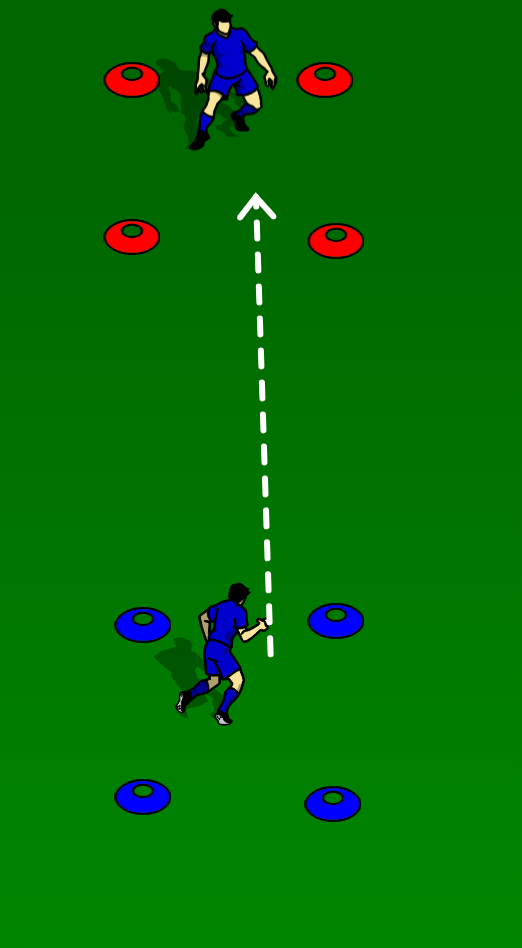
\includegraphics[width=.6\textwidth]{../img/Trimmed/Box_Passing}
        %    \caption{Drill: 4 Person Passing}
        %\end{figure}
    \end{minipage}
    \hspace{0.05\linewidth}
    \begin{minipage}{.6\linewidth} % Left column and width
        \textbf{Drill Description:}
        Place colored pairs of cones 2 yards apart over a 10x10 yard area.  Pair the players up and they are to pass to each other through the each gate.  They have to pass through each gate before they can pass through a second time.  Have them count the number of gates they passed through.
        
        \textbf{Coaching Points:}
        \begin{itemize}
        \setlength{\itemsep}{0pt}
        \setlength{\parskip}{0pt}
        \setlength{\parsep}{0pt}
        \item Technique:
        \begin{itemize}
            \setlength{\itemsep}{0pt}
            \setlength{\parskip}{0pt}
            \setlength{\parsep}{0pt}
            \item Step to the ball, planting the non-kicking foot next to the ball with toe pointed at the target.
            \item Use the inside of the foot to strike the middle of the ball.
            \item Follow through with the kicking foot.
        \end{itemize}
        \item The player without the ball should be moving more because they can move faster.
        \item Think of the cones as defenders - you want to position yourself in a manner that you split those defenders.
        \end{itemize}

    \end{minipage}
\end{minipage}

\end{oddBlock}